\documentclass[12pt]{report}

% includes
\usepackage{tikz}
\usepackage{amsmath}
\usepackage{float}
\usepackage{fancyvrb}
\usepackage{multirow}
\usetikzlibrary{shapes,arrows,positioning, fit}
\usepackage{geometry}           % page size
\usepackage[utf8]{inputenc}     % encoding
\usepackage{palatino}           % font
\usepackage[english]{babel}    % language
\usepackage{graphicx}           % images
\usepackage{indentfirst}        % indentation
\usepackage[nottoc]{tocbibind}  % table of contents style
\usepackage[unicode]{hyperref}  % references from the table of contents

% includes options
\geometry{  a4paper,            % scientific thesis standard
            left=3cm,
            right=2cm,
            top=2cm,
            bottom=2cm,
 }
\graphicspath{{images/}}        % path where the images are located
\setlength{\parindent}{1cm}     % paragraph indentation

% other options
\linespread{1.5}                % space between lines
\renewcommand*\contentsname{Cuprins}    % table of contents name

% the document content
\begin{document}
    % macros (global)
    \newcommand{\university}    {Universitatea "Alexandru-Ioan Cuza" din Iași}
\newcommand{\universityg}   {Universității "Alexandru-Ioan Cuza" din Iași} % genitive
\newcommand{\faculty}       {Facultatea de informatică}
\newcommand{\facultyg}      {Facultății de informatică} % genitive
\newcommand{\speciality}    {Securitatea Informatiei}
\newcommand{\promotion}     {2025}                                  %<---------

\newcommand{\thesistype}    {Lucrare de disertație}
\newcommand{\thesistitle}   {Streamlining Blockchain security audits through desktop applications}    %<---------

\newcommand{\authorlast}    {Enache-Stratulat}                               %<---------
\newcommand{\authorfirst}   {Marius}
\newcommand{\authornamefl}  {\authorfirst \space \authorlast} % first name first
\newcommand{\authornamelf}  {\authorlast \space \authorfirst} % last name first
\newcommand{\authorbirth}   {31 mai 2001}                      %<---------
\newcommand{\authoraddress} {România, jud. Bacău, mun. Bacău, strada Milcov, nr. 65, bl. 65, ap. 4} %<---------
\newcommand{\authorcnp}     {5010531046224}                         %<---------

\newcommand{\session}       {Iulie, 2025}                       %<---------
\newcommand{\coordinator}   {Conf. Dr. Andrei Arusoaie}               %<---------

\newcommand{\dottedline}    {............................}
    
    % front-matter
    \pagenumbering{gobble}
    
    % define the cover page
\begin{titlepage}
    \begin{center}
        % the university and faculty
        \large
        \MakeUppercase{\university}
        
        \LARGE
        \textbf{\MakeUppercase{\faculty}}
        
        % the faculty logo
        \vspace{1cm}
        
\includegraphics[width=0.3\textwidth]{logoFii.png}
        
        % thesis title
        \vspace{1cm}
        \Large
        \MakeUppercase{\thesistype}
        
        \vspace{0.5cm}
        \LARGE
        \textbf{\thesistitle}
        
        % author
        \vspace{2cm}
        \Large
        propusă de
        
        \vspace{0.5cm}
        \LARGE
        \textbf{\authornamefl}
        
        % session
        \vfill
        \Large
        \textbf{Sesiunea:} \session
        
        % scientific coordinator
        \vspace{2cm}
        \Large
        Coordonator științific
        
        \vspace{0.5cm}
        \LARGE
        \textbf{\coordinator}
    \end{center}
\end{titlepage}
    % define the title page
\begin{titlepage}
    \begin{center}
        % the university and faculty
        \large
        \MakeUppercase{\university}
        
        \LARGE
        \textbf{\MakeUppercase{\faculty}}
        
        % thesis title
        \vspace{8cm}
        \huge
        \textbf{\thesistitle}
        
        % author
        \vspace{2cm}
        \LARGE
        \textbf{\authornamefl}
        
        % session
        \vfill
        \Large
        \textbf{Sesiunea:} \session
        
        % scientific coordinator
        \vspace{4cm}
        \Large
        Coordonator științific
        
        \vspace{0.5cm}
        \LARGE
        \textbf{\coordinator}
    \end{center}
\end{titlepage}
    \vspace*{\fill}

\begin{flushright}
    Avizat, \\
    Îndrumător lucrare de disertație, \\
    \coordinator. \\
    Data: \dottedline \hspace{1cm} Semnătura: \dottedline
\end{flushright}

\vspace{1cm}
\begin{center}
    \large
    \textbf{Declarație privind originalitatea conținutului lucrării de licență}
\end{center}

Subsemnatul \textbf{\authornamelf} domiciliat în \textbf{\authoraddress}, născut la data de \textbf{\authorbirth}, identificat prin CNP \textbf{\authorcnp}, absolvent al \facultyg, \textbf{\faculty} specializarea \textbf{\speciality}, promoția \promotion, declar pe propria răspundere cunoscând consecințele falsului în declarații în sensul art. 326 din Noul Cod Penal și dispozițiile Legii Educației Naționale nr. 1/2011 art. 143 al. 4 și 5 referitoare la plagiat, că lucrarea de licență cu titlul \textbf{\thesistitle} elaborată sub îndrumarea domnului \textbf{\coordinator}, pe care urmează să o susțin în fața comisiei este originală, îmi aparține și îmi asum conținutul său în întregime.

De asemenea, declar că sunt de acord ca lucrarea mea de licență să fie verificată prin orice modalitate legală pentru confirmarea originalității, consimțind inclusiv la introducerea conținutului ei într-o bază de date în acest scop.

Am luat la cunoștință despre faptul că este interzisă comercializarea de lucrări științifice în vederea facilitării falsificării de către cumpărător a calității de autor al unei lucrări de licență, de diplomă sau de disertație și în acest sens, declar pe proprie răspundere că lucrarea de față nu a fost copiată ci reprezintă rodul cercetării pe care am întreprins-o.

\begin{flushright}
    Data: \dottedline \hspace{6cm} Semnătura: \dottedline
\end{flushright}

\vspace*{\fill}
\pagebreak
    \vspace*{\fill}
\begin{center}
    \large
    \textbf{Declarație de consimțământ}
\end{center}

Prin prezenta declar că sunt de acord ca lucrarea de licență cu titlul \textbf{\thesistitle}, codul sursă al programelor și celelalte conținuturi (grafice, multimedia, date de test, etc.) care însoțesc această lucrare să fie utilizate în cadrul \facultyg.

De asemenea, sunt de acord ca \faculty \space de la \university, să utilizeze, modifice, reproducă și să distribuie în scopuri necomerciale programele-calculator, format executabil și sursă, realizate de mine în cadrul prezentei lucrări de licență.

\begin{flushright}
    Absolvent \textbf{\authornamefl} \\
    \vspace{0.5cm}
    Data: \dottedline \hspace{6cm} Semnătura: \dottedline
\end{flushright}
\vspace*{\fill}
\pagebreak
    
    % table of contents
    \tableofcontents
    
    % chapters
    \setcounter{page}{1}
    \pagenumbering{arabic}
    
    \chapter*{Motivation} 
\addcontentsline{toc}{chapter}{Motivation}

The Blockchain Technology is relatively new if we consider the release of Bitcoin cryptocurrency blockchain newtork which took place in 2009. However, its foundation was formed decades ago, in 1989, when Leslie Lamport developed the Paxos protocol (to be continued...) 
    \begin{abstract}
    The Blockchain, despite its popularity and presence on the internet and in the financial sector, is a relatively new technology and this fact is proved by the large amount of attacks that took place on such networks. This situation raises the need for secure and robust networks that can keep the clients’ financial assets safe. Fortunately, there are various solutions to this category of problems, like Slither or Manticore, which take different approaches towards finding vulnerabilities. For the moment, most of these tools provide an at least decent detection for a high variety of attacks, but they need to get used more in order to ensure a higher standard of security when it comes to smart contracts. A good way to achieve this is to integrate the scanning tools into user-friendly applications that shorten the process of analyzing and fixing vulnerabilities.
\end{abstract}

\chapter*{Introduction} 
\addcontentsline{toc}{chapter}{Introduction}

The 21st century, so far, featured many advancements in the technology field. In the first decade, the internet had its peak spread among the high majority of people, the second one had seen a large grouth of the smartphone's adoption across the globe and now, in the third decade, the artificial intelligence is the most used and discussed breakthrough. The blockchain, while more nieche than the other technologies, also gained very much traction in the last 10 years, especially since 2020, when many people tried to take advantage of the sudden rise of Bitcoin, in both popularity and value, through mining or trading.

The blockchain is a decentralized, distributed and immutable ledger in which every user can add new blocks without the need of a central authority. Its foundation as a concept can be traced back to Leslie Lamport's Paxos protocol \cite{paxos}, released in 1998, which describes a system designed to achieve consensus among a network of computers, which is needed for agreeing on each iteration of the ledger, as it cannot be modified after its submission.

These systems, starting with the release of Ethereum, allowed the development of smart contracts \cite{smartContracts}, which are self-executing applications stored on the blockchain. The instructions of a smart contract are triggered when certain conditions are met and can be called without the need of a server. This property, along with its deterministic, transparent and immutable nature, gives the user the most power and responsability possible.

This technology has emerged only about 16 years ago, which can be seen because of the multitude of attacks that affected the networks that are based on it. This is why there is a need for secure and rezillient networks that can prevent the loss of clients' assets. Thankfully, there are many different tools that alleviate this concern, such as Slither \cite{slither} and Manticore \cite{manticore}, which find vulnerabilities in smart contracts in different ways. The aim of this thesis is to show Slither's strenghts and introduce SmartScan, an open-source desktop application that integrates it in a more seamless process of detecting and fixing security errors. This application is especially meant for students and aspiring smart contract developers.
    
    \chapter{Threats of Blockchain}
The Blockchain \cite{blockchainAttacks} is a technology used in various applications, such as cryptocurrencies, Internet of Things, electronic voting and many others. Its transparent, fully distributed, peer to peer and append-only nature are its most notable strengths. The transactions, which may have a different meaning depending on the application they are used for, are publicly visible and cannot be modified after they are published. This means the users may verify any transaction with no need of a centralized authority.

Bitcoin, the most popular cryptocurrency at this moment, takes advantage of these characteristics, creating a decentralized financial system. Unfortunately, there are also significant shortcomings in terms of security. One of the most notorious instances where these vulnerabilities had been exploited is known as ``The DAO'' \cite{blockchainAttacks}, where in 2016, an unknown attacker managed to drain \$50 million USD through a \textit{Reentrancy Attack}.

This thesis will first present the variety of attacks that blockchain networks are vulnerable to, their manner of work and potential effects to its victims. The Quadriga Initiative \cite{quadriga}  - a community-based platform - hosts a list of most of the attacks and frauds that involve cryptocurrency exchanges. Among the most well-known attacks, the database of case studies includes instances of Reentrancy Attacks, Replay Attacks and Short Address Attacks.

\textit{Reentrancy Attacks} \cite{reentrancy} can take place whenever the developers of the targeted network do not update the balances before sending the funds. In this case, an attacker could recursively call the withdraw() method and drain all the available funds. 

\textit{Replay Attacks} \cite{replay} are specific to the case where a cryptocurrency is forked into two separate currencies. In such a scenario, it is possible to sniff a regular transaction from any of the chains and “replay” it on the other. Processing both transaction causes the user to lose the same amount of assets twice (for example, paying two ether instead of one for the same product or service). This attack was easily possible in the Ethereum blockchain before the implementation of chainID in transactions.

\textit{Short Address Attacks} \cite{blockchainAttacks} represent the exploit of a bug in the EVM – Ethereum Virtual Machine – used to obtain extra tokens on purchases. This category of attacks requires creating an Ethereum wallet with its address ending with a 0 byte. The attacker makes a purchase on the address by removing the last digit and causes the contract to try to append the missing byte to the incomplete address, but it ends up appending it to the paid amount. In this case, the contract pays 256 times more tokens than intended. 

In terms of prevention and detection of such attacks, there are numerous tools that serve this purpose. As Kaixuan Li et al. describe in their article \cite{staticAnalysisToolsComparison}, a significant category of such tools detect vulnerabilities in the code through either static analysis or symbolic execution.


\begin{table}[h]
\centering
\begin{tabular}{cccc}
\hline
Technology         & Tool       & Analysis Level & Stars \\ \hline
                   & Securify2  &                & 529   \\
Static Analysis    & Slither    & Source Code    & 4 500 \\
                   & SmartCheck &                & 315   \\ \hline
                   & Manticore  &                & 3 500 \\
Symbolic Execution & Osiris     & Bytecode       & 50    \\
                   & Oyente     &                & 1 300 \\ \hline
\end{tabular}
\caption{List of the main static analysis and symbolic execution tools, adapted from Kaixuan Li et al. \cite{staticAnalysisToolsComparison}}
\end{table}

According to table 1.1, the static analysis tools, primarly represented by Slither, enjoy a higher popularity than the symbolic execution tools, represented by Manticore. This fact is shown by the number of stars on GitHub, which indicate how popular a tool is. These types of tools share the principle of scanning the code without executing it, but do so in different ways.

Generally, static analysis tools \cite{staticAnalysisDef} are automatic methods that determine the run-time properties of a program without running it. In Slither's \cite{slither} case, the analysis' purpose is to detect security vulnerabilities within the smart contract and to point out potential optimizations, which result in a lower gas consumption, an essential aspect in this field. As such, this category of security tools should be considered the opposite of Dynamic Analysis tools, which rely on running the target program and can also monitor it's performance among other aspects.

On the other hand, symbolic execution tools \cite{symbolicExecutionDef} take a similar approach of analyzing the given program without running the code, based solely on its bytecode. Esentially, Manticore \cite{manticore} uses the bytecode of a smart contract to map out all the execution paths of the program. Afterwards, all the paths get explored and the tool determines what kind of inputs determine each possible outcome. Two of the main components of Manticore are the Core Engine and the Event System. The Core Engine is responsible with operating and managing the state of a program at a certain point in the execution. The Execution Module has the purpose to emulate a system that runs the target program, with a CPU, system memory and an operating system like Linux.

\begin{figure}[H]
\centering
\begin{BVerbatim}
int foobar(int a, int b) {
    int x = 1, y = 0;
    if (a != 0) {
        y = 3 + x;
        if (b == 0) {
            x = 2 * (a + b);
        }
    }
    assert(x - y != 0);
}
\end{BVerbatim}
\caption{Example of code to analyze. From Roberto B et al. \cite{symbolicExecutionDef}}
\end{figure}

The figure above shows a simple example of function that a symbolic execution tool can operate on. A tool like Manticore can trace all the possible paths the execution may go at run-time. The assertion at the end is the possible point of failure for this function, in case \texttt{x} and \texttt{y} are equal.

\begin{figure}[H]
\centering
\resizebox{\textwidth}{!}{%
\usetikzlibrary{arrows.meta}

\begin{tikzpicture}[
  node distance=0.8cm and 1.6cm,
  every node/.style={font=\small},
  box/.style={rectangle, draw, rounded corners, align=left, text width=7cm, minimum height=1.2cm},
  ok/.style={ellipse, draw, align=center, minimum height=1cm, minimum width=2cm},
  error/.style={ellipse, draw=red, text=red, align=center, minimum height=1cm, minimum width=3.5cm},
  ->, >=Stealth
]

% Nodes
\node[box] (A) {\textbf{A}\\$\sigma = \{a \mapsto \alpha_a, b \mapsto \alpha_b\}$\\$\pi = \text{true}$\\2. int x = 1, y = 0};

\node[box, below=of A] (B) {\textbf{B}\\$\sigma = \{a \mapsto \alpha_a, b \mapsto \alpha_b, x \mapsto 1, y \mapsto 0\}$\\$\pi = \text{true}$\\3. if (a != 0)};

\node[box, below left=of B] (C) {\textbf{C}\\$\sigma = \{a \mapsto \alpha_a, b \mapsto \alpha_b, x \mapsto 1, y \mapsto 0\}$\\$\pi = \alpha_a \neq 0$\\4. y = 3 + x};

\node[box, below=of C] (E) {\textbf{E}\\$\sigma = \{a \mapsto \alpha_a, b \mapsto \alpha_b, x \mapsto 1, y \mapsto 4\}$\\$\pi = \alpha_a \neq 0$\\5. if (b == 0)};

\node[box, below=of E] (F) {\textbf{F}\\$\sigma = \{a \mapsto \alpha_a, b \mapsto \alpha_b, x \mapsto 1, y \mapsto 4\}$\\$\pi = \alpha_a \neq 0 \land \alpha_b = 0$\\6. x = 2 * (a + b)};

\node[box, below=of F] (H) {\textbf{H}\\$\sigma = \{a \mapsto \alpha_a, b \mapsto \alpha_b, x \mapsto 2(\alpha_a + \alpha_b), y \mapsto 4\}$\\$\pi = \alpha_a \neq 0 \land \alpha_b = 0$\\8. assert(x - y != 0)};

\node[error, below=of H] (ERR) {ERROR\\$2(\alpha_a + \alpha_b) - 4 = 0 \land \alpha_a \neq 0 \land \alpha_b = 0$ \\\\ $\text{if } \alpha_a = 2 \land \alpha_b = 0$};

\node[box, below right=of E] (G) {\textbf{G}\\$\sigma = \{a \mapsto \alpha_a, b \mapsto \alpha_b, x \mapsto 1, y \mapsto 4\}$\\$\pi = \alpha_a \neq 0 \land \alpha_b \neq 0$\\8. assert(x - y != 0)};

\node[ok, below=of G] (OKG) {OK\\$1 - 4 = 0 \land \alpha_a \neq 0 \land \alpha_b \neq 0 \Leftrightarrow \text{false}$};

\node[box, below right=of B] (D) {\textbf{D}\\$\sigma = \{a \mapsto \alpha_a, b \mapsto \alpha_b, x \mapsto 1, y \mapsto 0\}$\\$\pi = \alpha_a = 0$\\8. assert(x - y != 0)};

\node[ok, below=of D] (OKD) {OK\\$1 - 0 = 0 \land \alpha_a = 0 \Leftrightarrow \text{false}$};

% Edges
\draw[->] (A) -- (B);
\draw[->] (B) -- node[left] {$\alpha_a \neq 0$} (C);
\draw[->] (B) -- node[right] {$\alpha_a = 0$} (D);
\draw[->] (C) -- (E);
\draw[->] (E) -- node[left] {$\alpha_b = 0$} (F);
\draw[->] (E) -- node[right] {$\alpha_b \neq 0$} (G);
\draw[->] (F) -- (H);
\draw[->] (H) -- (ERR);
\draw[->] (G) -- (OKG);
\draw[->] (D) -- (OKD);

\end{tikzpicture}%
}
\caption{Example of symbolic execution tree of function \texttt{foobar}. Each state shows the symbolic store $\sigma$, the path constraint $\pi$, and the current statement. From Roberto B. et al \cite{symbolicExecutionDef}}
\end{figure}

As shown in this graph, $\sigma$ contains all the symbols stored in the context of the function, $\pi$ is a statement that represents the path constraint and below it is the line of code that gets excecuted at a given time. State \textit{B} is the first one to fork in two hypothetical states, based on the value of the first parameter, as shown by $\pi$ in the states \textit{C} and \texttt{D}. If \texttt{a == 0}, the function skips to the final assert and returns with no failure. Otherwise, the program would continue with state \texttt{E} and the following ones. Finally, a symbolic execution tool can reveal that the function will throw an error in case \texttt{a == 2 and b == 0}.

\begin{table}
\centering
\begin{tabular}{ccccl}
\hline
\multirow{2}{*}{Tool} & \multirow{2}{*}{\# Success} & \multicolumn{3}{c}{\# Failure}         \\ \cline{3-5} 
                      &                             & \# Timeout & \# Compilation & \# Total \\ \hline
Slither               & 767 (97.34\%)               & 2          & 19             & 21       \\
Manticore             & 112 (14.21\%)               & 626        & 50             & 676      \\ \hline
\end{tabular}
\caption{Success rate and failures summary of Slither and Manticore. Adapted from Kaixuan Li et al. \cite{staticAnalysisToolsComparison}}
\label{tab:my-table2}
\end{table}

Finally, to address Manticore's performance, as shown above, its exhaustive approach causes it to fail most of the tests due to timeout. Even if we were to ignore the timeout fails, Slither is visibly more consistent, having less compilation failures. The main flaw and reason of Manticore's high timeout rate may be the fact that it has to process large amounts of possible paths in order to find the ones where a security flaw is exploited. As such, Slither is the more consistent and better performing in comparison to Manticore.

\section{Slither}

Considering the performance metrics discussed in the first section, this section will be dedicated to Slither \cite{slither}, a static analysis tool catered to smart contracts written in Solidity and designed to offer granular information about smart contract code. This tool specializes in vulnerability detection, but also manages to point out potential optimizations that lower the gas consumption of a smart contract. In order to facilitate the usage of this tool, Slither leverages printers to help the user better understand the contract’s functionality and structure. This is done through representations such as the control flow graph or the inheritance graph or summaries of the contract and the issues detected in its code. 

In opposition to dynamic analysis \cite{dynamicAnalysis} tools, which rely on executing the contract’s code to find security weaknesses, static analysis tools detect vulnerabilities without running the smart contract. Such approaches include parsing and decompiling the EVM bytecode and translating it into semantic facts. These semantic facts are then matched with predefined patterns meant to reveal common issues.

Slither \cite{slither} proceeds in a similar manner by taking the Solidity Abstract Syntax Tree generated by the compiler and extracting information such as the control flow graph and transforms the code given into SlithIR, its internal representation language. After these two initialization stages, the actual code analysis takes place. In this stage, Slither identifies the reads and writes of variables, analyses the data dependency and determines whether the methods are protected from unauthorized use (for instance, only the owner of a contract may create new tokens).

This tool \cite{slither} helps auditors detect various vulnerabilities and potential security threats, such as reentrancy attacks or uninitialized storage variables. Its aproach of quickly transalating and analyzing large codebases makes it significantly faster than symbolic execution engines, as shown Table 1.2, a great feature for fast development workflows.

Furthermore, its set of detectors are able to find obvious and subtle vulnerabilities alike while providing useful educational resources to help developers fix and prevent future attacks. All these factors make Slither a great solution for quick and automated daily audit processes, preventing many critical security vulnerabilities.

Another essential topic in blockchain development, beside security concerns, is optimization, the techniques used to lower the ``gas'' consumption. Slither includes a set of detectors specialized in finding ways to optimize code \cite{slitherGitHub} from different perspectives. They are able to find issues such as dead code, as in methods or code branches that are never called or executed, unused state variables or variables that should be declared constant to save gas.

\begin{figure}[h]
    \centering
    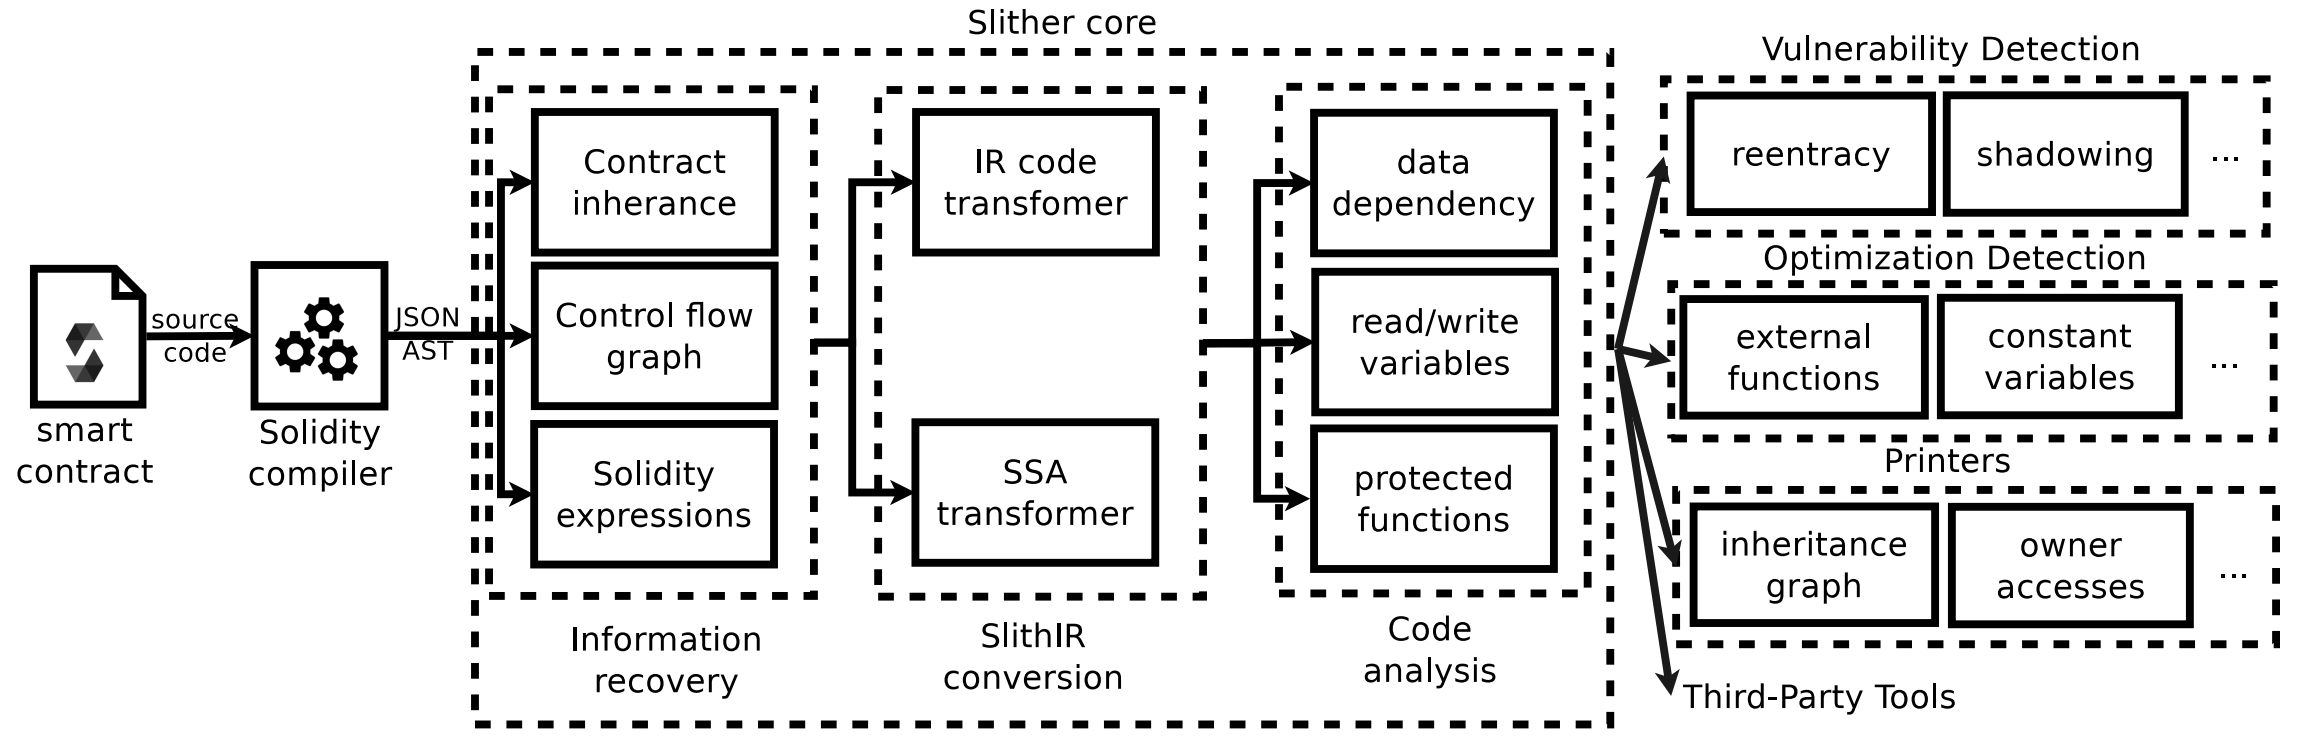
\includegraphics[width=1\linewidth]{images/image.png}
    \caption{Slither overview. From Josselin F. et al. \cite{slither}}
    \label{fig:enter-label}
\end{figure}

As to how it works \cite{slither}, Slither uses a multi stage procedure to parse and process the codebase of a blockchain project. First, it uses the Solidity compiler to generate the Abstract Syntax Tree of the contract, from which it recovers important information: inheritance graph, control flow graph and the list of expressions. Next, the contracts get translated to SlithIR, the internal representation language. The following step is the actual code analysis, in which Slither processes data dependencies, read/write variables and protected functions to output detected vulnerabilies and optimization opportunities. 

    \chapter{Slither's performance analysis}
This chapter will be dedicated to assessing Slither's performance in terms of vulnerability detection. The metrics used to determine how well security scanning tools work are: detection rate (how often a tool can correctly flag a vulnerability), analysis speed and attacks coverage (the variety of attacks that a tool can prevent).

\begin{table}[h]
\small
\begin{tabular}{cc|cccc|}
\cline{3-6}
                                                           &                         & \multicolumn{1}{c|}{Slither} & \multicolumn{1}{c|}{Securify} & \multicolumn{1}{c|}{SmartCheck} & Solhint       \\ \hline
\multicolumn{1}{|c|}{\multirow{3}{*}{Accuracy}}            & False Positive Rate     & 10.9\%                       & 25\%                          & 73.6\%                          & 91.3\%        \\
\multicolumn{1}{|c|}{}                                     & Flagged contracts       & 112                          & 8                             & 793                             & 81            \\
\multicolumn{1}{|c|}{}                                     & Detections per contract & 3.17                         & 2.12                          & 10.22                           & 2.16          \\ \hline
\multicolumn{1}{|c|}{\multirow{2}{*}{Performance}}         & Execution time  & 0.79 $\pm$ 1                   & 41.4 $\pm$ 46.3  & 10.9 $\pm$ 7.14                   & 0.95 $\pm$ 0.35 \\
\multicolumn{1}{|c|}{}                                     & Time out rate           & 0\%                          & 20.4\%                        & 4\%                             & 0\%           \\ \hline
\multicolumn{1}{|c|}{Robustness}                           & Failure rate            & 0.1\%                        & 11.2\%                        & 10.22\%                         & 1.2\%         \\ \hline
\multicolumn{1}{|c|}{\multirow{2}{*}{Reentrancy examples}} & DAO                     & Yes                          & No                            & Yes                             & No            \\
\multicolumn{1}{|c|}{}                                     & Spankchain              & Yes                          & No                            & No                              & No            \\ \hline
\end{tabular}
\caption{Performance comparison between Slither, Securify, SmartCheck and Solhint. From Josselin F. et al.\cite{slither}}
\label{tab:my-table}
\end{table}

The table above covers the first two performance criteria: the detection rate and analysis speed. The experiment was done by analyzing 1000 contracts focusing only on reentrancy detectors. Slither's results are visibly better than the ones obtained by its counterparts. Firstly, it's false positive rate is far lower, at just 10.9\%, while Securify falls in the second place with 25\%. Secondly, it's average execution time is also significantly lower than those of Securify and SmartCheck. In short, Slither is by far faster, more accurate and more consistent than the other three tools. Another important aspect is the time out rate of 0\% for Slither and Solhint, which further supports Slither's consistency in the detection of reentrancy attacks. Also, while this results do not conclude Slither's attack coverage, we can see it is the only tool that managed to detect attacks similar to the ones that targeted DAO or Spankchain, which are notorious for the amount of funds stolen and its effect on people's perception towards blockchain's security.

\begin{table}[h]
\centering
\begin{tabular}{|cccccc|}
\hline
\multicolumn{1}{|c|}{Vulnerabilities} & \multicolumn{1}{c|}{Read} & \multicolumn{1}{c|}{TP} & \multicolumn{1}{c|}{TN} & \multicolumn{1}{c|}{FP} & FN \\ \hline
\multicolumn{1}{|c|}{Re-entrancy}     & 29/31                     & 28                      & 0                       & 0                       & 1  \\
\multicolumn{1}{|c|}{Access Control}  & 18/18                     & 14                      & 0                       & 0                       & 3  \\
\multicolumn{1}{|c|}{Arithmetic}      & 15/15                     & 0                       & 0                       & 5                       & 0  \\
\multicolumn{1}{|c|}{Unchecked LLC}   & 26/26                     & 26                      & 0                       & 0                       & 3  \\ \hline
Total                                 & 88                        & 68                      & 0                       & 5                       & 7  \\ \hline
\end{tabular}
\caption{Slither's coverage of security attacks. Adapted from Senan B. \cite{staticAnalysisTest}}
\label{tab:my-table1}
\end{table}

This table shows how Slither can detect four types of vulnerabilities: Reentrancy, Access Control, Arithmetic and Unchecked LLC and covers 4 cases: True Positive(TP), True Negative(TN), False Positive(FP) and False Negative(FN). Out of the 90 test cases given, 88 passed the reading phase, 68 had got correctly flagged as vulnerable, five ended up as False Positives and seven as False Negatives. That equates to a rate of 77.27\% for True Positive, 5.68\% for False Positive and 7.95\% for False Negative. Therefore, while in almost 6\% of cases the user is falsely lead to believe a section of his code is vulnerable, a case that has no impact on the project's security, the rate at which Slither misses a vulnerability is almost 8\%. In particular, Slither missed 3.45\% of reentrancy attacks, 16.67\% of Access Contol attacks, none of the Arithmetic attacks and 11.54\% of Unchecked LLC attacks. As such, Slither may leave the analyzed project open to Access Control and Unchecked LLC attacks to a higher degree.
\section{Titlul secțiunii 1}

A diam sollicitudin tempor id eu nisl. Hac habitasse platea dictumst vestibulum. Integer enim neque volutpat ac tincidunt. Facilisi nullam vehicula ipsum a arcu cursus vitae congue. Vel turpis nunc eget lorem. Vestibulum mattis ullamcorper velit sed ullamcorper morbi tincidunt ornare. Nunc sed blandit libero volutpat. Sit amet luctus venenatis lectus magna fringilla urna porttitor. Hac habitasse platea dictumst quisque sagittis purus. Sed faucibus turpis in eu mi bibendum neque egestas. Vel orci porta non pulvinar neque laoreet suspendisse interdum consectetur. Erat nam at lectus urna duis convallis convallis tellus id. Tristique sollicitudin nibh sit amet commodo nulla facilisi nullam vehicula. Etiam dignissim diam quis enim lobortis scelerisque. Nunc congue nisi vitae suscipit tellus mauris a diam maecenas. Lacus viverra vitae congue eu consequat ac felis donec. Mauris sit amet massa vitae tortor condimentum. Mauris augue neque gravida in. Lorem ipsum dolor sit amet. Arcu dui vivamus arcu felis bibendum ut tristique et.

\section{Titlul secțiunii 2}

Sit amet mauris commodo quis imperdiet massa tincidunt nunc pulvinar. Ligula ullamcorper malesuada proin libero nunc consequat interdum. Mauris a diam maecenas sed enim ut. Ut sem nulla pharetra diam sit amet nisl suscipit adipiscing. Leo duis ut diam quam nulla. Neque ornare aenean euismod elementum. Vitae sapien pellentesque habitant morbi tristique senectus. Lectus magna fringilla urna porttitor rhoncus dolor purus non enim. Egestas sed sed risus pretium quam vulputate dignissim suspendisse in. At quis risus sed vulputate odio ut enim. Hac habitasse platea dictumst quisque sagittis. Lectus vestibulum mattis ullamcorper velit sed. Massa vitae tortor condimentum lacinia quis vel eros donec ac. Vulputate dignissim suspendisse in est ante. Sed faucibus turpis in eu mi bibendum neque. Enim eu turpis egestas pretium aenean pharetra magna. Tellus mauris a diam maecenas.

\section{Titlul secțiunii 3}

Faucibus ornare suspendisse sed nisi lacus sed. Mi in nulla posuere sollicitudin aliquam ultrices. Lacus suspendisse faucibus interdum posuere lorem ipsum dolor sit amet. Odio tempor orci dapibus ultrices in iaculis nunc sed augue. Congue eu consequat ac felis donec et odio. Enim ut sem viverra aliquet eget sit amet. Sit amet consectetur adipiscing elit duis tristique sollicitudin. Quis blandit turpis cursus in. Cras fermentum odio eu feugiat pretium nibh ipsum consequat nisl. Non curabitur gravida arcu ac tortor dignissim convallis aenean. Porta non pulvinar neque laoreet suspendisse interdum consectetur libero id. Lacus viverra vitae congue eu consequat ac felis. Vulputate dignissim suspendisse in est ante in nibh mauris. Amet mauris commodo quis imperdiet massa. Varius sit amet mattis vulputate enim nulla aliquet. Pellentesque diam volutpat commodo sed egestas egestas. Amet est placerat in egestas erat imperdiet sed euismod. Scelerisque varius morbi enim nunc faucibus a pellentesque sit. Ut sem viverra aliquet eget sit amet tellus cras. Sem integer vitae justo eget magna fermentum iaculis eu.
    \chapter{SmartScan}

SmartScan is a desktop application that aims to help begginer developers evaluate their projects from a security standpoint while it can also help regular users evaluate how safe a smart contract is. The main purpose of this project is to be easy to use, but also powerful enough to provide relevant insight and guidance towards fixing the security vulnerabilities. For this purpose, SmartScan uses the GitHub REST API \cite{gitHubRestAPI} for a quick and intuitive project cloning process and Slither \cite{slitherGitHub} for the analysis of the cloned project.

The choice for the analysis tool was not difficult for multiple reasons, as conveyed by the previous chapter. The first one is in its core design: being a static analysis tool makes it great for scanning projects without executing them, which would have added complexity to the entire setup. Secondly, its balance between high performance and low execution time in terms of scanning for security threats is great for providing fast and reliable vulnerability reports.

\begin{figure}[h]
    \centering
    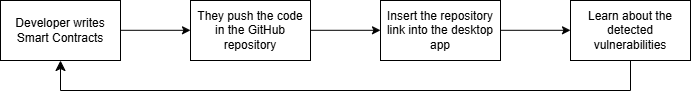
\includegraphics[width=1\linewidth]{images/scenario-diagram.png}
    \caption{Scenario diagram for SmartScan.}
    \label{fig:enter-label}
\end{figure}

As shown in the diagram above, the usual workflow in which SmartScan is involved starts with the developer writing the smart contract code and pushing it in the GitHub repository. Out application intervenes right after, when the developer copies the repository link in it and starts the analysis. Afterwards, the application returns a security report, based on which the developer may start fixing the vulnerabilities and the cycle may repeat. Whenever the application runs the analysis, it makes sure to fetch the latest version of the project so the developer doesn't need to.

\begin{figure}[h]
    \centering
    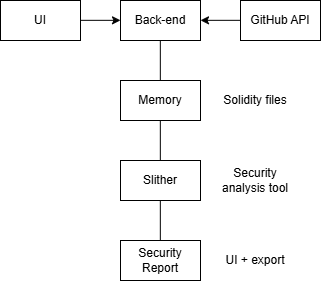
\includegraphics[width=0.5\linewidth]{images/component-diagram.png}
    \caption{Component diagram for SmartScan.}
    \label{fig:enter-label}
\end{figure}

In terms of infrastructure and design choices, SmartScan is developed in Python, using the PySide 6 framework \cite{pySide6} for the interface because it provides a clean and easy to use design with minimal performance limitations. The back-end of the application consists of the aforementioned REST API and Slither, linked together with custom scripts designed to manage the analysis results.

\begin{figure}[h]
    \centering
    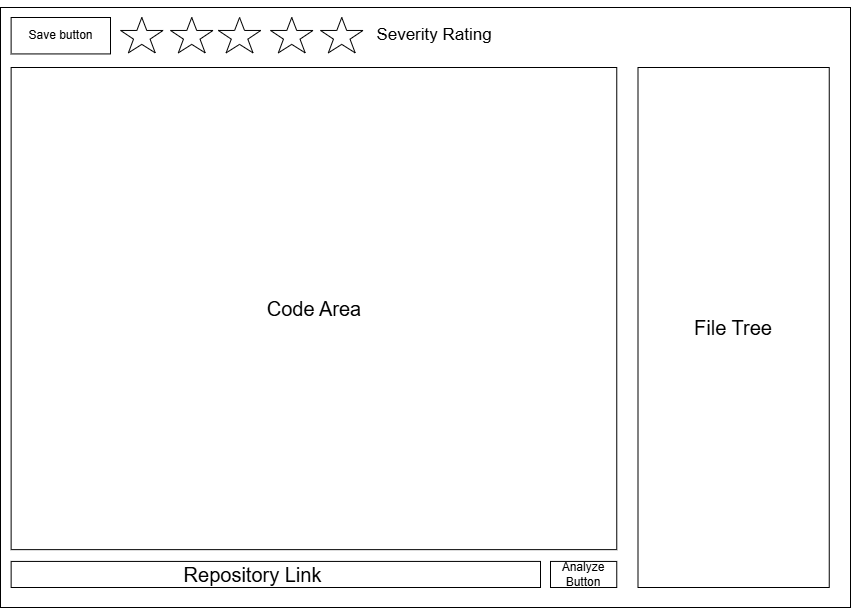
\includegraphics[width=0.80\linewidth]{images/application-design.png}
    \caption{SmartScan's User Interface.}
    \label{fig:enter-label}
\end{figure}

The figure above presents the user interface of SmartScan. The first component the user will interact with is the Repository Link text box, in which they will insert the repository link copied from GitHub before pressing the Analyze Button. Afterwards, the REST API will handle the cloning of the project and Slither will analyze it, returning all the found vulnerabilities. The File Tree is used to access the cloned project and open any Solidity file in order to see the code inside. The Code Area will host the code of the currently open file, with a side bar that shows the number of each line and a yellow highlight that shows which lines of code are vulnerable, as detected by Slither. The side bar and the highlight are meant to visually guide the developer towards the problem with ease. After fixing the code, the user may save the file through the dedicated button on the top left corner.

SmartScan, while using external APIs for cloning and analyzing the project, compiles a security report of its own, based on the vulnerabilities found by Slither. The whole report will be saved in a separate text file, so the user can access it whenever they want, and will be shown in the Code Area at the end of the analysis. Also, the stars next to the Save Button will turn red depending on the determined severity of the project. The metric used to measure how vulnerable a project is will be the amount of threats found and their severity. Each star turning red represents a higher vulnerability of the project as a whole. Ideally, the analyzed project should get a rating of zero stars, while a five-star rating is the worst case possible.

\begin{table}[h]
\centering
\begin{tabular}{|c|c|}
\hline
Star rating & Condition                                                              \\ \hline
0 $\star$   & No vulnerability found                                                 \\ \hline
1 $\star$   & $\leq 10$ vulnerabilities, no high severity ones                       \\ \hline
2 $\star$   & $\leq 25$ vulnerabilities, $\leq 2$ of high severity, no critical ones \\ \hline
3 $\star$   & $> 25$ vulnerabilities, $\leq 5$ of high severity, no critical ones    \\ \hline
4 $\star$   & $\leq 10$ high vulnerabilities or $\leq 2$ critical ones               \\ \hline
5 $\star$   & $> 10$ high vulnerabilities or $> 2$ critical ones                     \\ \hline
\end{tabular}
\caption{Project vulnerability rating done by SmartCheck.}
\label{tab:my-table}
\end{table}

A zero-star rating is obtained if Slither finds no security issue (informational and optimization issues are not included). A One-star rating is awarded if Slither finds less than 10 vulnerabilities, none of which are of high or critical severity. For a project to get a three-star rating, the project is required to have no critical vulnerability, but is allowed to have up to five high severity vulnerabilities. If any critical vulnerability is found, the project will get a rating of four or five stars regardless of how many issues are found.

The idea behind this rating is to raise awareness to the developer towards the security threats and induce a sense of urgency towards solving the high and critical vulnerabilities. For this reason, any critical vulnerability found will grant a minimum of four stars, while projects with no high severity vulnerabilities will only get one star. Furthermode, while one could argue that the rating should factor in the project's complexity and allow more vulnerabilities for larger projects, we should also consider that high-scale projects may also get targeted more often by attackers while the financial stakes are also higher. As such, the state of a project's security should not be influenced by its size.


\begin{figure}[h]
    \centering
    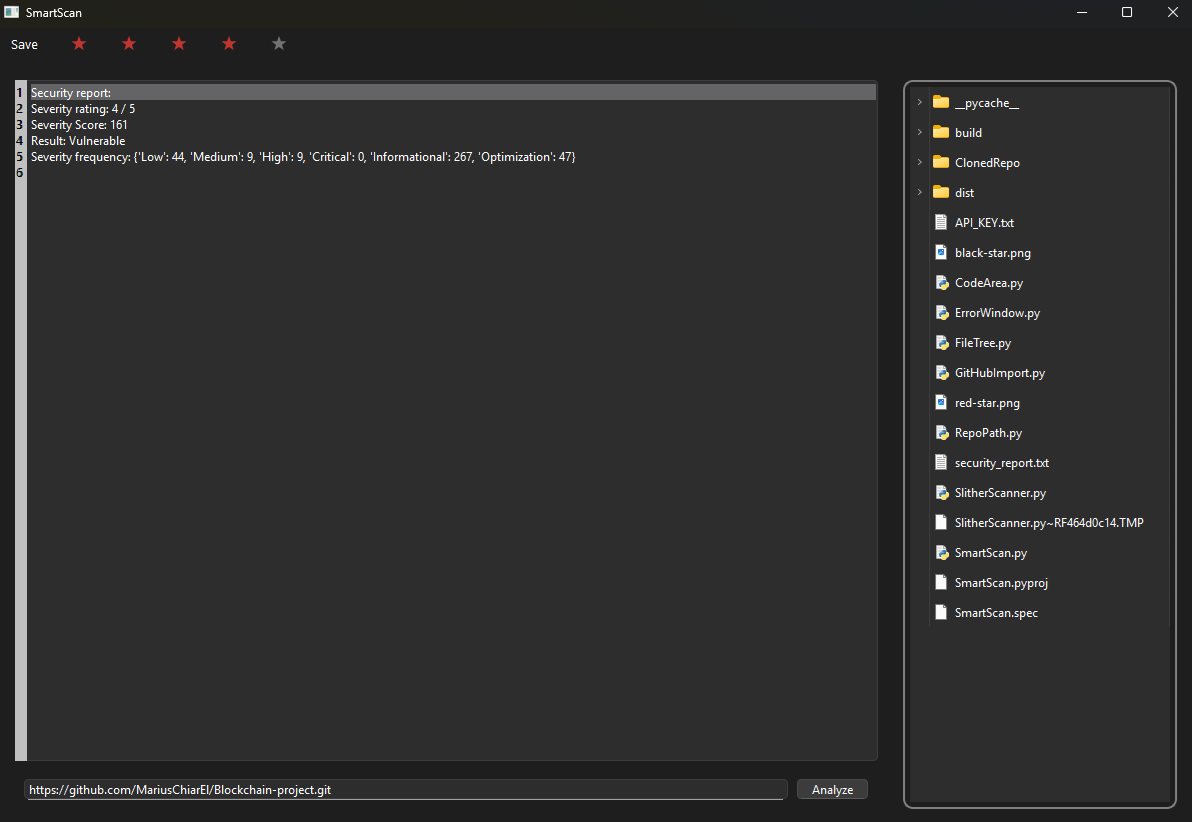
\includegraphics[width=1\linewidth]{images/application-design-in-practice.png}
    \caption{SmartScan's User Interface in practice: The Code Area features the final security report of a smart contract.}
    \label{fig:enter-label}
\end{figure}

As shown in the screenshot above, our sample smart contract project obtained a rating of four stars. Despite having no critical security issue, the high severity vulnerabilities are the root cause of these results. In this project, Slither had found 44 low severity errors, nine of medium severity and another nine of high severity. Additionally, the tool found 47 opportunities to optimize the smart contract and 267 informational errors, which are often not indicating any direct problems for the end user.

\begin{figure}[h]
    \centering
    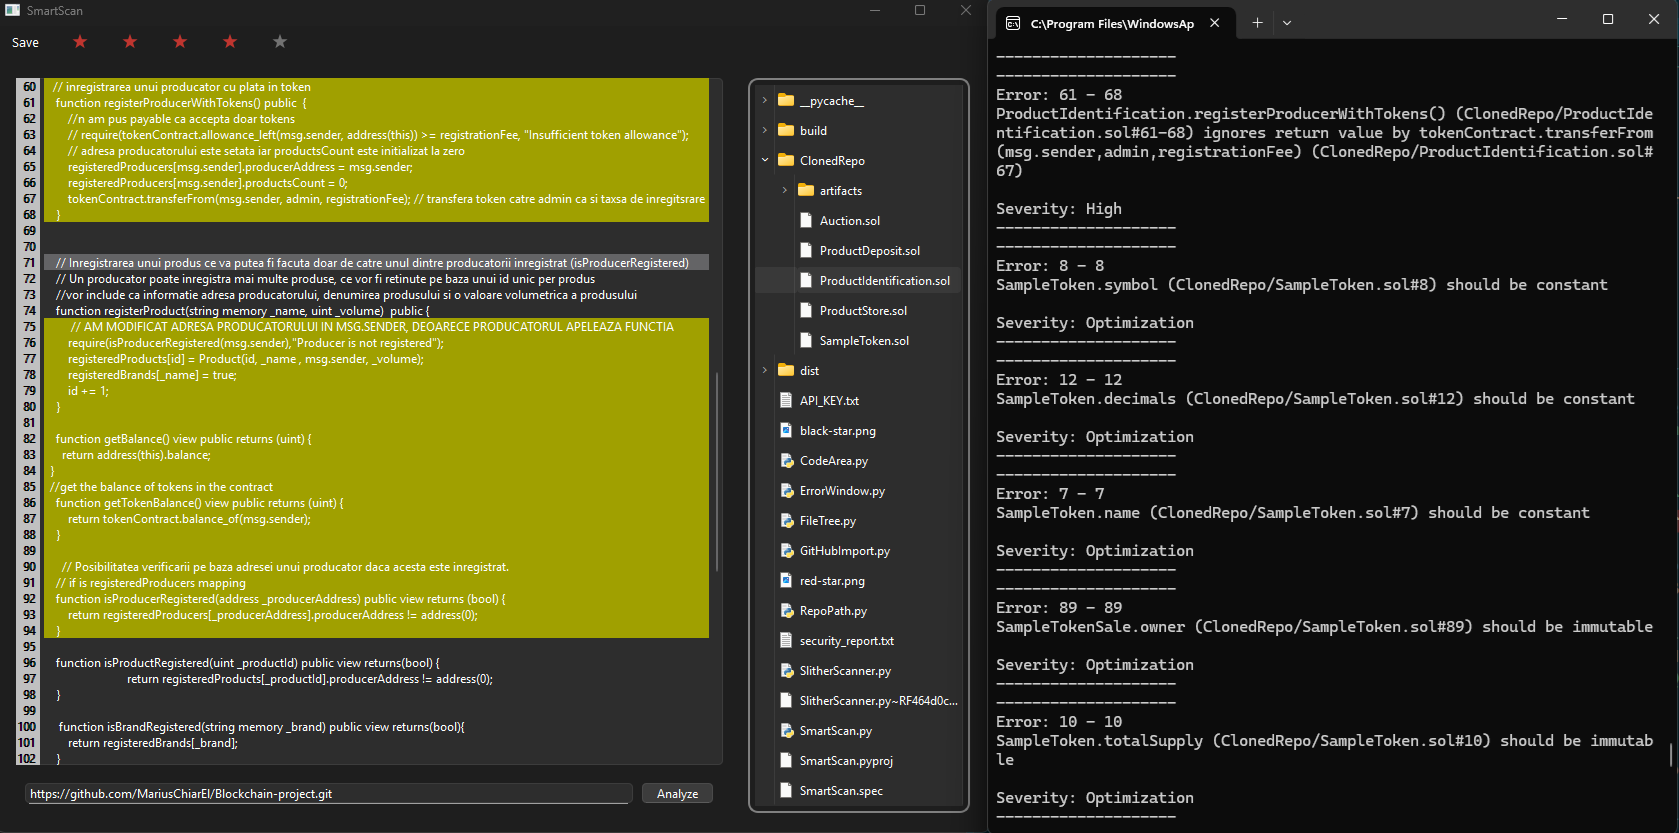
\includegraphics[width=1\linewidth]{images/highlighted-errors.png}
    \caption{SmartScan's User Interface in practice: The Code Area features the code of a Solidity file with its affected lines highlighted. The console shows the description of each error.}
    \label{fig:enter-label}
\end{figure}

The figure above shows SmartScan in action, highlighting the errors, as reported in the console. For instance, we can see the \texttt{registerProducerWithTokens()} method, containing an error at line 67, where \texttt{transferFrom()}\cite{solidityDocs} was called. Slither detected that this function had been called without checking its result, as it returns a boolean that tells whether the transfer succeeded. In this case, the registration proceed while the user does not have the funds to do so. This vulnerability has a high severity because any user can obtain the producer title without paying the smart contract as intended. This kind of vulnerability has the highest impact on the smart contract owner because they are the one to not get the funds they should have.

\begin{table}[h]
\begin{tabular}{cc|ccccc|}
\cline{3-7}
                                  &                                               & \multicolumn{5}{c|}{Errors (by severity)}                                                                                  \\ \hline
\multicolumn{1}{|c|}{Project}     & Overall Security Rating                       & \multicolumn{1}{c|}{Low} & \multicolumn{1}{c|}{Medium} & \multicolumn{1}{c|}{High} & \multicolumn{1}{c|}{Critical} & Total \\ \hline
\multicolumn{1}{|c|}{Project \#1 \cite{sampleProject1}} & 4/5 $\star$             & \multicolumn{1}{c|}{44}  & \multicolumn{1}{c|}{9}      & \multicolumn{1}{c|}{9}    & \multicolumn{1}{c|}{0}        & 62    \\
\multicolumn{1}{|c|}{Project \#2 \cite{sampleProject2}} & 3/5 $\star$             & \multicolumn{1}{c|}{16}  & \multicolumn{1}{c|}{10}     & \multicolumn{1}{c|}{3}    & \multicolumn{1}{c|}{0}        & 29    \\
\multicolumn{1}{|c|}{Project \#3 \cite{sampleProject3}} & 5/5 $\star$             & \multicolumn{1}{c|}{31}  & \multicolumn{1}{c|}{0}      & \multicolumn{1}{c|}{11}   & \multicolumn{1}{c|}{0}        & 21    \\ \hline
\end{tabular}
\caption{The security reports of three similar smart contracts.}
\label{tab:my-table}
\end{table}

This table shows the results SmartScan obtained by analyzing three similar smart contracts. The first one shows the highest amount of errors, caused primarily by the 44 low severity errors, but did not surpass the five star threshold of 10 high severity errors, so it earned four out of five stars. The second project shows the best results, having only three high severity vulnerabilities and a three star rating. At the same time, while it has the least total errors, the third project has the most high severity errors, which grant it the 5 star rating.

SmartScan achieves its goals to ease the audit process and guide its users to easily track the detected errors and optimizations by automizing most of the work, compiling an overall security report and highlighting the affected sections of the code while also naturally integrating into the development and testing process. Its qualities make it suitable in an academic setting, used by the students to see various coding patterns that lead to security vulnerabilities or inefficient usage of gas, or in a team of begginer developers who wish to provide the most secure solutions for their users. However, there are also multiple ways to improve the application and the user's experience. Firstly, a very useful feature would be generating a separate file that organizes the errors and helps the developer track the errors even more easily and to which they can add other errors, found through manual analysis or with the help of other tools. Additionally, after the project gets its errors fixed, Smart Scan could integrate the functions to review the differences, commit and push the improved code back to the repository to make the process as seamless as posiible. Another improvement of this application can take the form of a separate window that shows the last clicked error so they can easily see the errors one by one.

%[IDEA: SmartScan can generate a .json report of all the errors for the developer to track. If possible, the user should be able to insert their own found errors to keep track of.]
%[IDEA: SmartScan can be used by students to pinpoint the security flaws in their projects (educational use case)]

%[Future work / Good to have additions: highlight different severity vulnerabilities with different colors (gradient from yellow to red), use git.diff, separate window that shows the error in the affected code under the cursor, making it a web application or a VS Code extension]
    
    \chapter*{Concluzii} 
\addcontentsline{toc}{chapter}{Concluzii}

This thesis gravitated around three main subjects: blockchain's infrastructure, Slither's design and perfromance analysis and SmartScan, the application made to ease the security analysis process. Now we have a better picture of what blockchain is and how it functions, including qualities and shortcomings alike, potential attacks that affect this kind of networks and the currently available solutions to prevent them. The second chapter was dedicated to Slither, one of the best tools for security analysis, with emphasys on its infrastructure, functionality and performance compared to similar solutions. Lastly, we have introduced SmartScan, the application that integrates Slither to automatically detect vulnerabilities in remote projects. The description of SmartScan includes its infrastructure, feature set, workflow and examples of security reports generated by it. Our hope is that our contribution will enable aspiring developers to create secure smart contracts and that the blockchain will be safer to use in the long term as a consequence.

In conclusion, the blockchain is a very promising technology, with essential applications in various domains that evenly distributes the power and responsability to all its users. However, its security concerns keep its popularity low among most people and more security measures must be taken in order to restore its image and make it usable in key areas, such as electronic voting, which could significantly improve the voting process by easing it for both the citizens and the states. Nevertheless, there is a long road ahead of blockchain towards achieving its potential and it will need a lot of support from the scientific community for that to happen, much like any other new piece of techonology.

%chapter 1
%- scurta descriere blockchain, ce face bine si ce nu
%- cateva atacuri asupra blockchain
%- ce unelte exista pentru analiza securitatii si care s cele mai populare
%- ce tipuri de astfel de unelte exista si cum functioneaza

%chapter 2
%- ce este Slither si cum functioneaza
%- performana lui Slither in diverse scenarii
%- detectia e optimizari a lui Slither (mentionata)
%- consideratii etice in folosirea Slither

%chapter 3
%- ce este si cum functioneaza SmartScan
%- ce aduce in plus
%- care ar fi fluxul e lucru
%- componentele din care e format
%- sistemul de rating al securitatii proiectului
%- exemplu pentru functiile implementate
%- exemplu de raport de securitate pe 3 proiecte asemanatoare
%- cum poate fi folosit si unde ar excela
%- idei de imbunatatiri
    % Example citation to ensure at least one \cite command
    \cite{example_reference}
    \bibliographystyle{plain}
    \bibliography{chapters/bibliography}
\end{document}
